\section{Introduction}
\label{sec:intro}
% \varun{diff models are awesome! need a sentence + cite for that. However, .. }
Text-to-image diffusion models~\citep{ho2020denoising, rombach2022high, saharia2022photorealistic} have rapidly become the dominant generative paradigm for high-fidelity image synthesis, with deployments ranging from creative tools to commercial APIs.
% are increasingly subject to \varun{subject to is strong? perhaps we can say that this is an active area of research} 
Privacy concerns and copyrights have motivated active research on \emph{concept unlearning}~\citep{gandikota2023erasing}: given a trained model and an undesirable concept (e.g., an object category, an artistic style, or a specific identity), the goal is to suppress the concept while preserving the model's general capabilities. In this work, we focus on object-category concepts, where benchmarks and detectors are most mature.
% \varun{you say a bunch of different things are technically a concept, but you only evaluate "object category"? someone might find this problematic, so i would be a little more precise?} 
% deemed undesirable, unlearning methods seek to suppress the model's ability to generate that concept while preserving its overall generative utility.
% \varun{cites for diffusion unlearning?}. 
% \varun{what is a concept?} 
A growing body of work has proposed methods for this task, ranging from fine-tuning-based approaches that permanently alter model weights~\citep{gandikota2023erasing,fan2023salun,zhang2024defensive,srivatsan2025stereo} to inference-time interventions that block concept-specific activations without modifying the underlying model~\citep{li2024get,lyu2024one,cywinski2025saeuron}. These methods are typically evaluated on two families of metrics: \emph{unlearning accuracy} (UA), measuring whether the target concept has been successfully suppressed, and \emph{retain accuracy} (RA), measuring whether the model's performance on non-target concepts remains intact.

% \varun{can compress this para a lot!} 
A tacit assumption in this evaluation paradigm is that UA and RA can be optimized independently. However, our empirical evidence suggests this assumption is violated (\cref{sec:motivation}). Methods achieving strong erasure (high UA), such as STEREO~\citep{srivatsan2025stereo}, often degrade generation quality on semantically related concepts (low RA).
Methods with better retention, such as SAeUron~\citep{cywinski2025saeuron}, leave the target concept reachable through prompts that omit its name but supply correlated context (e.g., generating a horse from ``a jockey at the racetrack''), a phenomenon we call \emph{concept leakage}, resulting in low UA.
% \varun{what a correlated prompt is has not been introduced, so need a different (detailed) explanation here}. 
These observations indicate a fundamental tension: \emph{unlearning and retention are inherently coupled when concepts share representational structure}, a coupling visible directly in the model's internal representations, where semantically related concepts (\texttt{horse}/\texttt{pony}/\texttt{donkey}) occupy overlapping regions of activation space while isolated concepts (\texttt{castle}) sit well-separated (\cref{fig:umap_kappa}). 
This shows that concept activation regions are real geometric structures whose overlap reflects semantic similarity, motivating our formal notion of concept activation regions in~\cref{sec:tradeoff}\footnote{The formal definition of concept activation regions is in Appendix~\ref{app:concept_regions}; full empirical construction details and per-concept clustering statistics are in Appendix~\ref{app:activation_regions}.}.
Two failure modes follow from this geometry: \emph{concept leakage}, where the target concept reappears under indirect prompts, and \emph{collateral forgetting}, degraded generation of semantically related but distinct concepts. We show that these are not shortcomings of individual algorithms but dual symptoms of overlapping concept regions, and that any robust erasure method must trade them off.

\begin{figure*}[t]
\centering
\begin{minipage}[c]{0.55\linewidth}
\centering
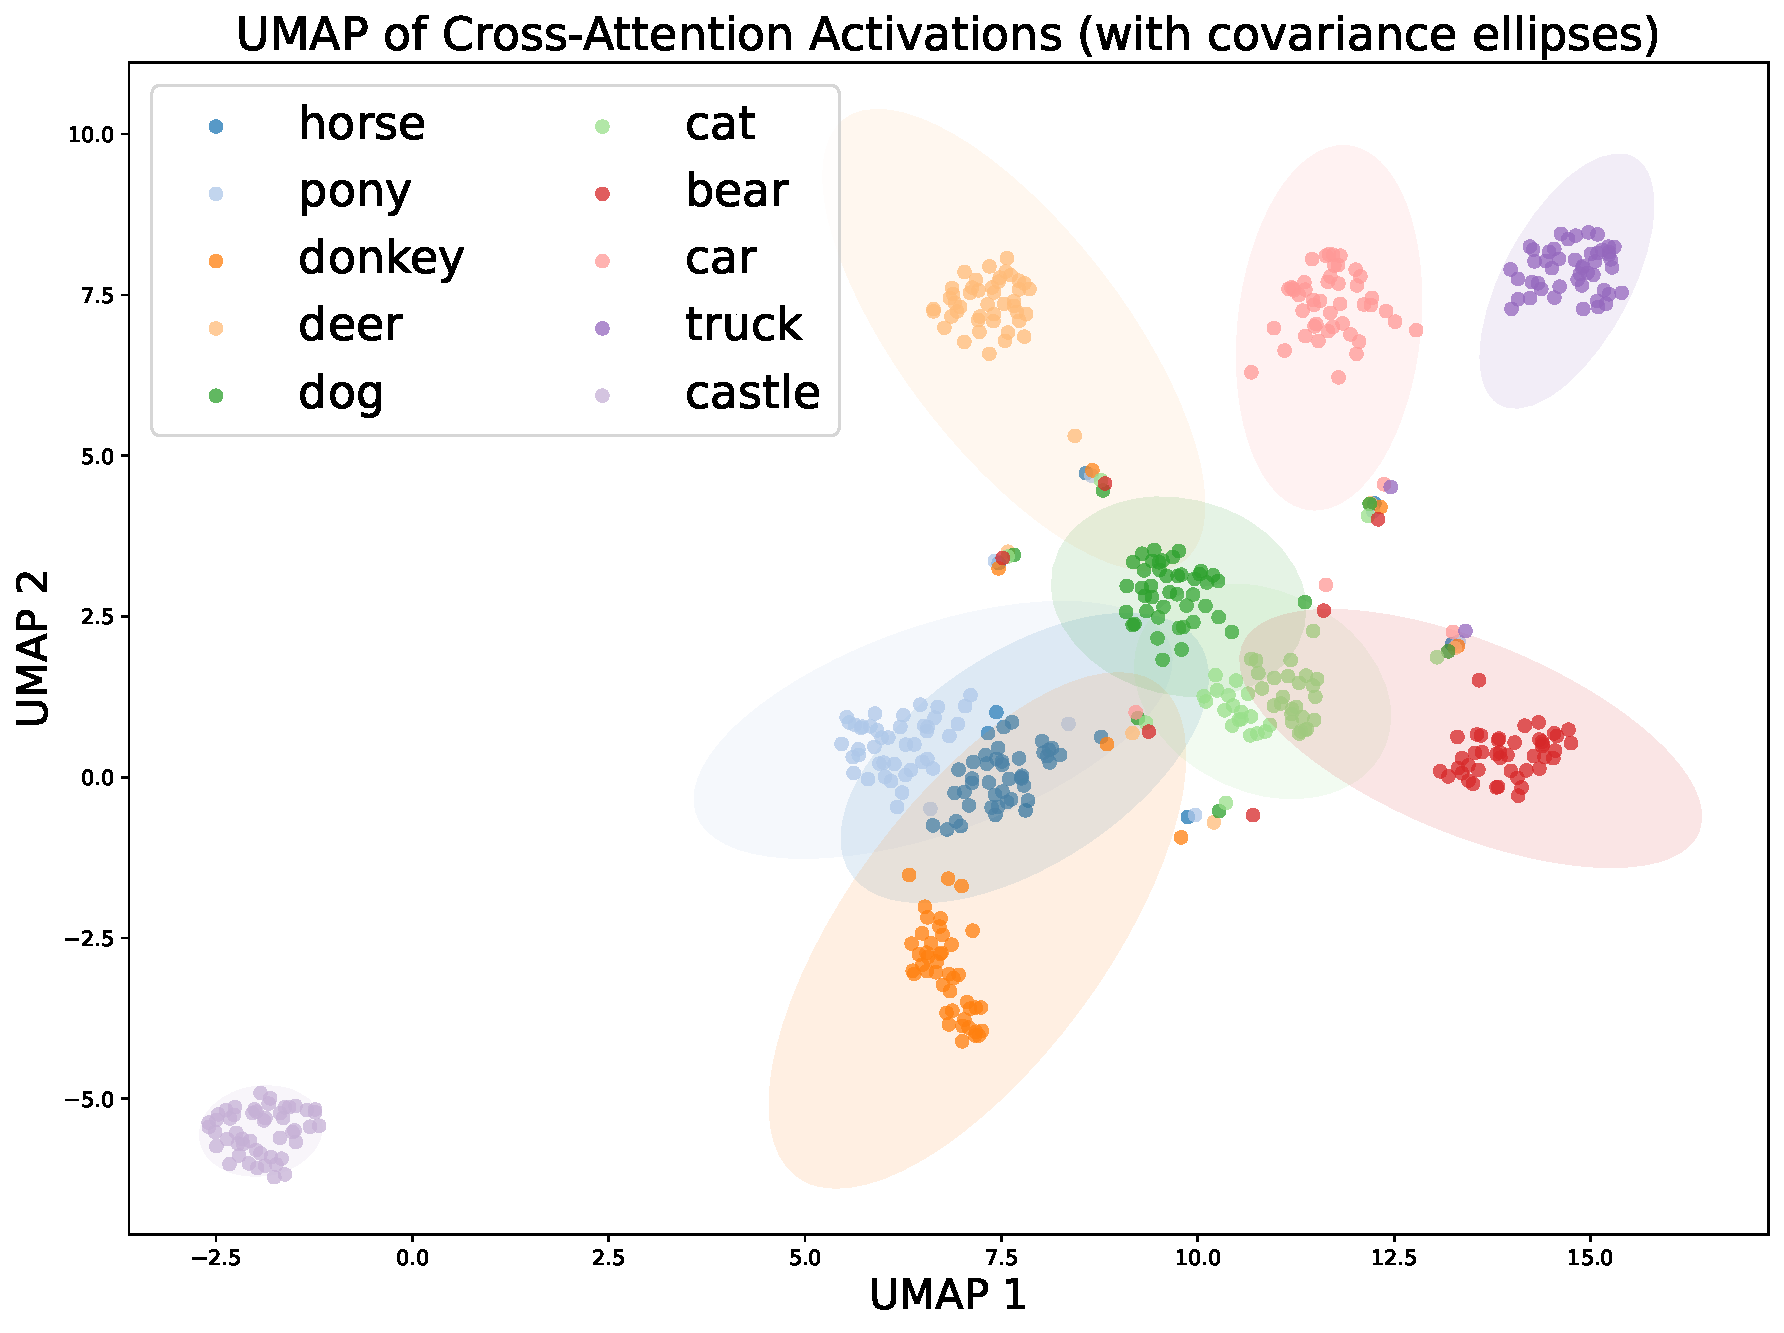
\includegraphics[width=\linewidth]{img/umap_v3_ellipses.pdf}

\vspace{6pt}

\small
\setlength{\tabcolsep}{6pt}
\begin{tabular}{lcl}
\toprule
Concept & $\hat\kappa$ & Neighbors \\
\midrule
dog    & 0.89 & puppy, labrador \\
bear   & 0.82 & black bear, grizzly \\
horse  & 0.81 & donkey, foal, mare \\
cat    & 0.77 & kitten, panther \\
castle & 0.27 & fortress, palace, citadel \\
\bottomrule
\end{tabular}
\end{minipage}\hfill
\begin{minipage}[c]{0.42\linewidth}
\caption{\textbf{Concepts occupy coherent, partially overlapping regions in activation space.}
\emph{Top-left:} UMAP projection of cross-attention activations at \texttt{mid\_block.attentions.0} (step 25/50) for 10 concepts in Stable Diffusion v1.4 (visualization pool; full evaluation pool in~\Cref{app:vocab}); each point is one prompt and ellipses show 95\% covariance contours. Semantically related concepts (\texttt{horse}/\texttt{pony}/\texttt{donkey}) cluster together, while isolated concepts (\texttt{castle}) are well-separated.
\emph{Bottom-left:} Estimated entanglement coefficient $\hat\kappa$ (fraction of the target's activation region shared with semantic neighbors; see~\cref{def:overlap}). The Neighbors column lists representative discovered neighbors; full per-target neighbor sets are reported in~\cref{app:kappa_estimation}. Animal subtypes have high $\hat\kappa$ and dense neighbor sets; \texttt{castle} has low $\hat\kappa$ despite a comparable number of architectural neighbors.}
\label{fig:umap_kappa}
% Aliases preserve existing \cref{fig:umap} and \cref{tab:kappa} references elsewhere in the paper; all three labels resolve to this combined float.
\label{fig:umap}
\label{tab:kappa}
\end{minipage}
\end{figure*}

\paragraph{Contributions.} 
\textbf{(i)} We give a geometric account of concept entanglement, showing that the literature's two failure modes, 
% \varun{earlier, you called this concept leakage; be consistent?}
concept leakage and collateral forgetting, are dual symptoms of overlapping concept regions in cross-attention activation space (quantified by an entanglement coefficient $\hat\kappa$), rather than separate algorithmic shortcomings as treated in prior work~\citep{gandikota2023erasing,zhang2024defensive,srivatsan2025stereo,cywinski2025saeuron}. \textbf{(ii)} Building on this account,
% we prove a method-agnostic lower bound
we derive a geometric lower-bound for concept unlearning under empirically-verified assumptions: any method achieving $\varepsilon$-robust erasure must incur utility preservation error $\gamma \geq \kappa(1-\varepsilon)/L$ (\Cref{thm:tradeoff}), with strict impossibility at $\varepsilon = 0$ whenever $\kappa > 0$ (\Cref{cor:impossibility}); this result reframes unlearning as a Pareto problem rather than a dual-objective one. \textbf{(iii)} We validate the predicted $\kappa$-scaled trade-off across seven methods and five concepts spanning a wide range of $\hat\kappa$ values, using a new Neighbor Preservation metric tied to the activation-level $\gamma$ in our theorem.

% In this work, we argue that the UA/RA coupling observed above is not a shortcoming of individual unlearning algorithms but a structural consequence of how concepts are represented in diffusion models. 
% Our approach proceeds in three steps.
% First, we provide empirical evidence that concepts are represented as distributed patterns across correlated tokens, leading to both \emph{concept leakage}, the target concept reappearing under indirect prompts and \emph{collateral forgetting}, degraded generation of semantically related but distinct concepts (\Cref{sec:trade-off}).
% % \varun{what is this? undefined} (\Cref{sec:trade-off}).
% Second, we formalize this phenomenon by introducing concept activation regions and proving that achieving robust erasure necessarily incurs error in preserving remaining concepts (\Cref{sec:motivation}).
% Third, we empirically validate this trade-off across seven unlearning methods, revealing a Pareto frontier between erasure strength and utility preservation (\Cref{sec:experiment}).

% \varun{i still think we don't need this blurb, and it can be merged with the previous paragraph! will give you space for something downstream}

% We make three contributions. \textbf{(i) Concept entanglement in diffusion models:} we show that visual concepts are distributed across correlated tokens, causing concept leakage and collateral forgetting. \textbf{(ii) A fundamental unlearning--retention trade-off:} we prove that $\varepsilon$-robust concept erasure necessarily incurs non-zero error in preserving neighboring concepts, establishing that perfect unlearning and perfect retention cannot be achieved simultaneously. \textbf{(iii) Empirical characterization:} we benchmark seven unlearning methods and observe a consistent Pareto frontier between erasure strength and neighbor preservation.

 

% \varun{you can compress this full paragraph into 1-2 lines and add it to the previous paragraph, as the caption contains a lot of relevant details}
% To further probe the internal structure underlying these effects,~\cref{fig:umap} visualizes cross-attention activations for multiple concepts in Stable Diffusion. The resulting clusters show that prompts associated with the same concept occupy coherent regions in activation space, while concepts with nearby activation centroids in the extracted cross-attention space from neighboring clusters \ali{the second sentence seems to be incomplete?}. For example, \texttt{horse}, \texttt{pony}, and \texttt{donkey} form a dense equine cluster, while \texttt{castle} is well-separated from all animal concepts. 



% \varun{but who decides these are semantically related? you are making an informed decision; it is not learnt in some unsupervised manner?} 
% \begin{figure}[t]
% \centering
% 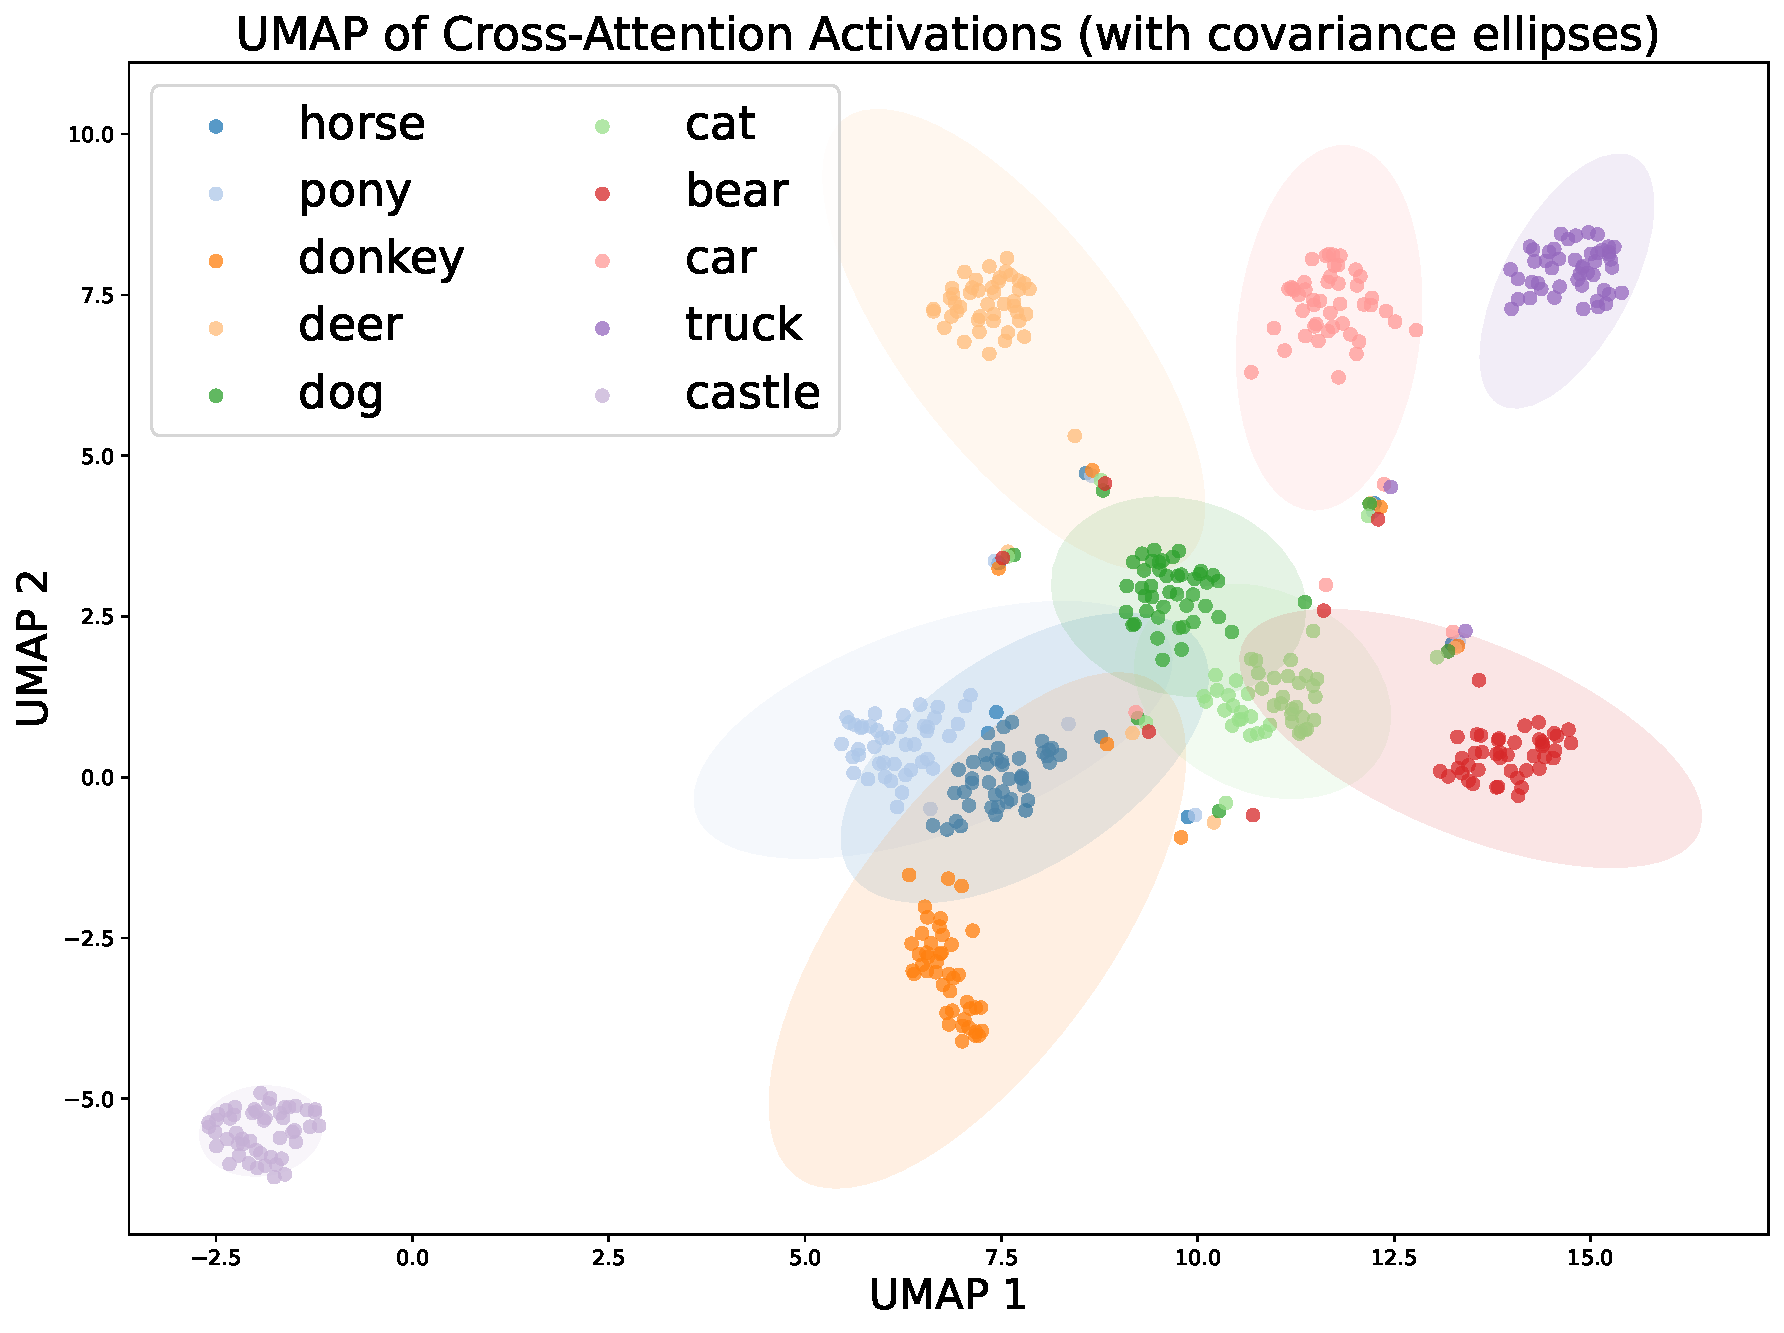
\includegraphics[width=0.6\linewidth]{img/umap_v3_ellipses.pdf}
% \caption{
% UMAP projection of cross-attention activations at \texttt{mid\_block.attentions.0} (step 25/50) for 10 concepts in Stable Diffusion v1.4. Each point corresponds to one prompt; ellipses show 95\% covariance contours. Semantically related concepts (\texttt{horse}/\texttt{pony}/\texttt{donkey}) cluster together, while isolated concepts (\texttt{castle}) are well-separated, confirming that concept activation regions (\Cref{def:activation}) are coherent, localizable structures. 
% % \varun{can make caption scriptsize; can also make the figure a "wrapfig" so that it occupies less space; in that case: please make the legend bigger?}
% % \ali{maybe instead of wrap figure, you can make a single figure side by side with Figure 2 and reduce the size of their captions (captions are too long i think) }
% % \ali{deer in this figure seems to be isolated from horse as well, but in the section for Effect 2, we are claiming that unlearning horse leads to collateral damage on related concepts such as deer. So either the figure needs adjustment or the text and examples.} \yian{I'll adjust the text part in appendix}
% % \varun{+1 for ali's suggestion, but with table 1 instead of fig 2}}
% \label{fig:umap}
% \end{figure}

% \varun{would remove the contributions bullets to save space}
% \paragraph{Contributions.} Our main contributions are:
% \begin{itemize}
% \item \textbf{Concept entanglement in diffusion models.}
% We show that visual concepts are distributed  across correlated tokens, causing concept leakage and collateral forgetting.
% \item \textbf{A fundamental unlearning--retention trade-off.}
% We prove that $\varepsilon$-robust concept erasure necessarily incurs non-zero error in preserving neighboring concepts, establishing that perfect unlearning and perfect retention cannot be achieved simultaneously.
% \item \textbf{Empirical characterization of the trade-off.}
% We benchmark seven unlearning methods and observe a consistent Pareto frontier between erasure strength and neighbor preservation.
% \end{itemize}


\begin{comment}
\varun{which section are these results in?}
First, we provide \textbf{empirical evidence of concept entanglement} in diffusion models (\S\ref{sec:trade-off}). We demonstrate that visual concepts are not represented as isolated, token-aligned features in the model's joint text--image space, but instead emerge from distributed co-occurrence patterns across correlated tokens. This entanglement has two observable consequences that are, in fact, two sides of the same coin: (i) \emph{concept leakage}---an erased concept can be regenerated through semantically related prompts that omit the target token; and (ii) \emph{collateral forgetting}---aggressively suppressing one concept damages the model's ability to generate neighboring concepts whose activation regions overlap with the target. We show both effects empirically across multiple unlearning methods.

\varun{which section are these results in?}
Second, we \textbf{formalize the robustness--retention trade-off} as a provable impossibility result (\S\ref{sec:motivation}). Working in the model's internal activation space, we define concept activation regions, their semantic neighborhoods, and an overlap coefficient $\kappa$ that quantifies the degree of entanglement between a target concept and its neighbors. Under mild continuity assumptions, we prove that any unlearning method achieving $\varepsilon$-robust erasure of a target concept must incur neighbor preservation error of at least $\gamma \geq \kappa \cdot (1-\varepsilon)/L - \delta$ (Theorem~\ref{thm:tradeoff}), where $L$ is a Lipschitz constant and $\delta$ captures the activation-space distance between concepts. A direct corollary establishes that \emph{simultaneous perfect erasure and perfect retention is impossible} whenever the target concept has nonzero overlap with its semantic neighborhood (Corollary~\ref{cor:impossibility}). This result provides a formal explanation for why existing methods are forced to navigate a Pareto frontier rather than achieve ideal performance on both axes.

\varun{which section are these results in?}
Third, we conduct a \textbf{comprehensive empirical study of the trade-off across seven unlearning methods} (\S\ref{sec:experiment}), spanning both fine-tuning-based and inference-time approaches. Using the \textsc{UnlearnCanvas} benchmark~\citep{zhang2024unlearncanvas}, we evaluate each method not only on standard UA, IRA, and CRA metrics but also on a new \emph{neighbor preservation} metric that measures collateral damage on semantically related concepts. Our results reveal a clear Pareto frontier: methods that achieve stronger erasure---particularly those employing adversarial training for robustness---systematically incur greater collateral damage on neighboring concepts, while inference-time methods that preserve neighbors more faithfully tend to leave residual pathways through which erased concepts can be recovered. We further show that the severity of the trade-off is governed by the semantic density of the target concept's neighborhood, consistent with the predictions of our theoretical framework.

\varun{maybe remove this below, as the previous 3 paragraphs are all contributions?}
\paragraph{Contributions.} Our main contributions are:
\begin{enumerate}
    \item \textbf{A formal impossibility result.} We prove that $\varepsilon$-robust concept erasure necessarily incurs neighbor preservation error lower-bounded by the concept overlap coefficient $\kappa$, establishing that the robustness--retention trade-off is a structural property of entangled concept representations, not an artifact of suboptimal algorithm design.
    
    \item \textbf{Empirical Pareto frontier.} We benchmark seven concept unlearning methods on both erasure completeness and neighbor preservation, revealing a consistent trade-off curve and identifying the mechanism-level factors (weight modification scope, intervention granularity) that determine where each method falls on this frontier.
    
    \item \textbf{Unified perspective on concept leakage and collateral forgetting.} We show that these two previously separate failure modes---vulnerability to indirect prompts and degradation of related concepts---are dual consequences of concept entanglement, providing a coherent framework for understanding and evaluating unlearning methods.
\end{enumerate}
\end{comment}
